\chapter{Theoretische Grundlagen}
\label{cha:Grundlagen}
In diesem Kapitel werden theoretische Grundlagen erläutert, die zum weiteren Verständnis der Arbeit benötigt werden. Zuerst werden ausgewählte Video-Schnittstellen erläutert, verglichen und bewertet um den praktischen Nutzen dieser für handelsübliche embedded Linuxsysteme aufzuzeigen. Im Weiteren werden zwei Linux Boards verglichen und bewertet, sowie deren praktische Einsatzgebiete beispielhaft dargelegt.

\section{Video-Schnittstellen}
Unter Schnittstellen sind die Berührungspunkte zweier Systeme zu verstehen, die der gemeinsamen Kommunikation dienen. Video-Schnittstellen verbinden Systeme und ermöglichen die Anzeige von Bilddaten. Dabei wird sie zur physikalischen Verbindung eines Systems mit einer Anzeigeeinheit verwendet. In der Video-Schnittstelle können sowohl Hardware- als auch Softwarekomponenten enthalten sein.
\subsection{VGA}
Beim Video Graphics Array handelt es sich um einen Grafik-Standard, der 1987 von IBM entwickelt wurde. Ein VGA-Stecker hat 15 Pins und liefert neben analogen Farbinformationen horizontale und vertikale Synchronisationssignale. Aufgrund der limitierten Spezifikationen ist die Schnittstelle eher \textit{veraltet} und selbs Intel als Chiphersteller will ab 2015 darauf verzichten und digitalen Schnittstellen den Vortritt lässt (\cite{Intel2010}). Zwar ist die VGA-Schnittstelle noch nicht komplett obsolet, so wird sie den digitalen Schnittstellen trotzdem weichen müssen. Heutige embedded Linuxsysteme zeigen, dass diese direkt mit HDMI oder anderen digitalen Schnittstellen entwickelt werden.
Die Funktionsweise der VGA-Schnittstelle ist in \refa{fig:vga_timing} zu sehen (siehe: \cite{Valcarce2011}). Es werden fünf analoge Leitungen benötigt: \code{R}, \code{G}, \code{B}, \code{HSYNC}\footnote{HSYNC: Horizontale Synchronisation} und \code{VSYNC}\footnote{VSYNC: Vertikale Synchronisation}. Die ersten Drei stellen die Farbwerte Rot, Grün und Blau dar. Je nach Intensität lassen sich aus einer Mischung der Farbkanäle die verfügbaren Farben darstellen. Zur Variation der Intensität können Pegel zwischen 0\,V (absolut dunkel) und +0.7\,V (absolut hell) angenommen werden. Die Signale \code{HSYNC} und \code{VSYNC} werden zur Steuerung der Zeilen und Spalten verwendet. Das Signal \code{HSYNC} zeigt an, wann eine Zeile vollständig abgetastet ist. Zwischen zwei \code{HSYNC}-Pulsen werden für jeden Pixel der Zeile zeitlich exakt Spannungen auf den Farbleitungen gelegt. Sind alle Zeilen eines Bildes komplett geschrieben, wird das \code{VSYNC}-Signal getriggert, welches den Start eines neuen Bilds einleitet und den Prozess von vorne beginnen lässt (\cite{Valcarce2011}).

\begin{figure}[htp]
	\centering
\fbox{	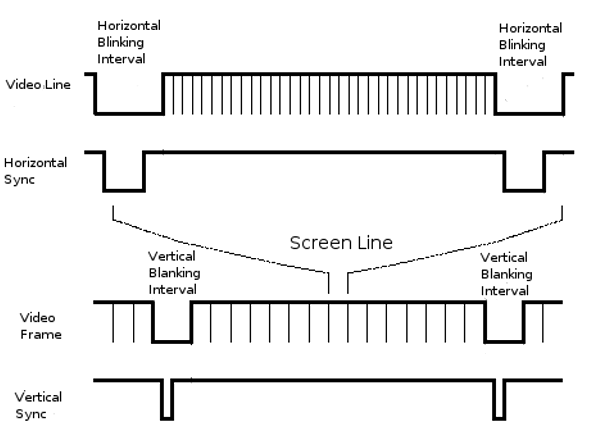
\includegraphics[width=0.7\textwidth]{Grundlagen/vga_timing.png}}
	\caption{VGA-Timing}
	\label{fig:vga_timing}
\end{figure}

\subsection{DVI}
Hinter DVI steht der Begriff Digital Visual Interface, welcher eine digitale Schnittstelle zur Grafikanzeige bezeichnet. Der DVI Standard wurde 1999 von der DDWG\footnote{DDWG: Digital Display Working Group} verabschiedet, da der Wunsch nach leistungsstärkeren Schnittstellen vorhanden war. QXGA-Auflösungen\footnote{QXGA: 2048x1536} sind z.\,B. auf analogem Wege nicht mehr befriedigend erzielbar. Die DVI Schnittstelle beinhaltet neben den digitalen Signalen zusätzlich analoge VGA Signale, was den Betrieb älterer Monitore und Displays zulässt. Zur digitalen Datenübertragung wird der TMDS-Standard\footnote{TMDS: Transition Minimized Differential Signaling - Differentielle Datenübertragung} verwendet, welcher die 24\,Bit Farbinformationen\footnote{24 Bit: je 8 Bit für Rot, Grün und Blau} mittels eines \code{Serializers} in serielle Daten umwandelt. Je nach benötigter Bandbreite können drei oder sechs Aderpaare für Pixeldaten verwendet werden. Dies wird Single- bzw. Dual-Link genannt. Es lassen sich dabei maximal 3.72 GBit/s\footnote{max. UXGA: 1600x1200@60Hz} bzw. 7.44 GBit/s\footnote{max. WUXGA: 1920x1200@60Hz} übertragen. Um die Paare zuordnen zu können, wird ein weiteres Paar zur Synchronisation des Taktes verwendet. Damit die Übertragung noch effizienter gestaltet werden kann, gibt es die Möglichkeit bei High- sowie Low-Pegel des Taktsignals Daten zu übertragen\footnote{\textit{Double Data Rate}} (\cite{Leunig2002}).

\subsection{HDMI}
Gegenüber der DVI-Schnittstelle bietet die HDMI-Schnittstelle dieselben Eigenschaften bezüglich der Videoübertragung und verwendet ebenfalls TMDS. Hinzu kommt allerdings, dass sowohl Audio als auch Ethernet unterstützt werden. Die Baugröße der Stecker ist für den Hausgebrauch verkleinert worden. HDMI wurde als normierte Universallösung entwickelt und hat sich als solche etabliert (\cite{Extron2014}). Nahezu jedes neu entwickelte Gerät mit Anzeigemöglichkeit bietet eine HDMI-Schnittstelle - ebenso embedded Linux Boards, wie z.\,B. \code{Raspberry Pi} oder \code{BeagleBone Black}.

\subsection{RGB}
Der RGB-Bus wird für für kleine TFT-Panels bis ca. 10\,Zoll verwendet und funktioniert prinzipiell analog zur VGA-Schnittstelle. Der Unterschied ist hierbei, dass die Datenleitungen komplett digital arbeiten. So werden die Signale für rot, grün und blau nicht mehr analog im Bereich von 0\,V bis +0.7\,V dargestellt, sondern durch einen üblicherweise acht Bit breiten Bus pro Farbkanal. Die Auflösung pro Farbe ist mit 255 Intensitätsstufen ausreichend, um ein Farbspektrum von 16.777.216 Farben\footnote{16.777.216 Farben = $2^{24}$} zu erhalten. 
\begin{figure}[htp]
	\centering
\fbox{	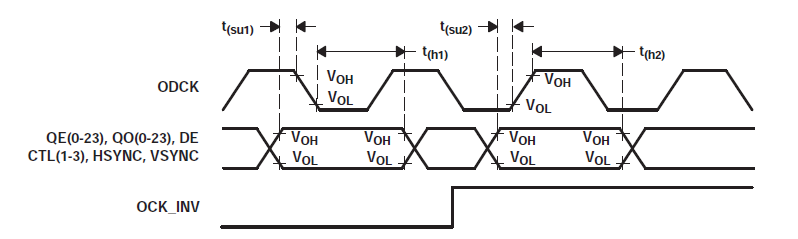
\includegraphics[width=0.8\textwidth]{Grundlagen/rgb_timing.png}}
	\caption{RGB-Timing}
	\label{fig:rgb_timing}
\end{figure}
Dieser Farbmodus wird auch RGB888 genannt, da acht Bit für jede Farbe zur Kodierung, insgesamt 24 Bit, zur Verfügung stehen. Neben dem 24 Bit Modus ist RGB565 (je fünf Bit für Rot und Blau und sechs Bit für Grün) noch weit verbreitet. Hier ergibt sich ein Farbspektrum von 65.536 Farben\footnote{65.536 = $2^{16}$}. Da digital übertragen wird, ist eine Taktleitung notwendig, um die Synchronität zu gewährleisten. 
Aufgrund der Verbreitung und Mächtigkeit der Schnittstelle besitzen einige Prozessoren, wie z.\,B. der Linux-fähige OMAP3530 von Texas Instruments, eine RGB-Schnittstelle. 
\refa{fig:rgb_timing} zeigt exemplarisch ein Timing-Diagramm der RGB-Schnittstelle des Bausteins TFP-401A von Texas Instruments (siehe: \cite{TI2011}).
\subsection{LVDS}
Um lange Strecken und hohe Auflösungen übertragen zu können, ist der parallele Datentransfer ungeeignet, da bei schnellem Takt z.\,B. der Einfluss von Störungen zu groß und das Signal schneller beeinträchtigt wird. Deshalb ist die Praktik, große Datenmengen über eine differentielle Hochgeschwindigkeits-Verbindung wie z.\,B. LVDS\footnote{LVDS: Low Voltage Differential Signaling} zu übertragen, beliebt. Die physikalische Funktionsweise besteht darin, dass zweimal dasselbe Signal, einmal mit positivem und einmal mit negativem Spannungspegel, übertragen wird. Wirkt nun von außen eine Störung auf die LVDS Leitung, werden beide Leitungen im gleichen Maße gestört. Durch das Zusammenführen beider Signale am Ende kompensieren sich diese Störungen im Idealfall zu Null. Das zuvor genannte TMDS arbeitet ähnlich, da es sich hierbei ebenfalls um eine differentielle Übertragungsart handelt. TMDS wird oft eingesetzt, sobald das Signal das Gerät verlässt - z.\,B. Desktop-Bildschirm mit Anschlusskabel. Befindet sich das Anzeigegerät allerdings im selben Gehäuse, so wird häufig LVDS eingesetzt. Neben Bilddaten ist es natürlich auch möglich andere Nutzdaten wie z.\,B. Messwerte von Sensoren zu übertragen. 
Aufgrund der hohen Geschwindigkeit und geringen Fehlerrate werden differentielle Übertragungen gerne für Displays angewendet.
\subsection{8080-Interface}
Das 8080-Interface ist eine antike Schnittstelle, welche ursprünglich vom Intel 8080 Prozessor herrührt. Sie wird bis heute verwendet, um Speicher, kleine TFT-Displays oder andere Bausteine mit einem Mikrocontroller zu betreiben. Das 8080-Interface besteht aus einem Daten- als auch einem Adressebus mit z.\,B. acht, 16 oder 32 Bit, je einer Leitung für Read-Enable, Write-Enable und Chip-Select. Durch die Verwendung der Chip-Select Leitungen ist es möglich, mehrere Teilnehmer am selben Bus zu betreiben. Alle Teilnehmer, deren Chip-Select-Leitung nicht aktiv ist, verhalten sich für andere Busteilnehmer unsichtbar. Erst mit Aktivierung der Chip-Selects werden diese sichtbar und übernehmen den Bus. Ein Hostsystem steuert als sog. Master die am Bus hängenden Slaves. Möchte das Hostsystem Daten lesen, wird mit der Chip-Select Leitung ein Lesezyklus initiiert die gewünschte Adresse an den Bus anlegt, die Read-Enable Leitung aktiviert und nach einer festgelegten Zeit diese wieder deaktiviert. Der Slave legt die gewünschten Daten auf den Datenbus und der Host kann diese Daten lesen. Analog dazu funktioniert der Schreibzyklus. 
\refa{fig:8080_timing} zeigt das Timing Diagramm eines Schreib- und Lesezyklus des Displaycontrollers SSD1289 (siehe \cite{SSD2007}). Das Signal \code{D/}\codeinvers{C} wird verwendet, um zu unterscheiden, ob Daten oder ein Kommando auf dem Bus anliegen und wird im Folgenden auch \code{RS} genannt. Dazu kann beispielsweise eine Adressleitung des 8080-Bus verwendet werden. \codeinvers{CS} stellt das Chip-Select dar. \codeinvers{WR} und \codeinvers{RD} beziehen sich auf Write- bzw. Read-Enable. \code{D0-D17} sind 18 Datenbits des Bus. 

\begin{figure}[htp]
	\centering
\fbox{	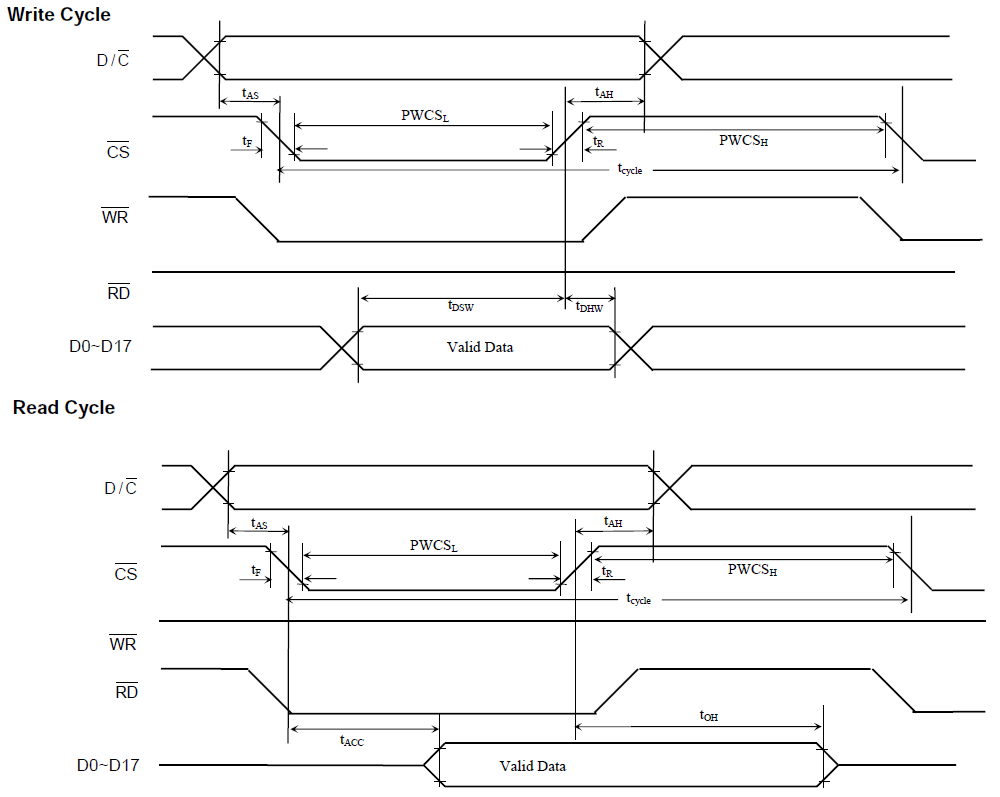
\includegraphics[width=1.0\textwidth]{Grundlagen/8080_timing.png}}
	\caption{8080-Timing des SSD1289}
	\label{fig:8080_timing}
\end{figure}
Viele Mikrocontroller besitzen bereits ein 8080-Interface in Hardware. Verfügt ein Controller nicht über diese Schnittstelle, kann das Protokoll mittels GPIO\footnote{GPIO: General Purpose In/Output} in Software implementiert werden. 
Da GPIO-Pins nicht für schnelles Schalten optimiert sind, ist dies allerdings wesentlich langsamer als eine Lösung, die bereits in Hardware realisiert ist.

\subsection{Bewertung der Video-Schnittstellen}
\label{cha:bewertung_video}
Nachdem nun die wichtigsten Schnittstellen dargestellt wurden, werden diese im Folgenden, mit dem Fokus auf die Relevanz hinsichtlich der Verwendung in dieser Arbeit, bewertet.
Da die VGA-Schnittstelle antik und obsolet ist, spielt sie heutzutage nur noch eine geringe Rolle. Insbesondere im Bereich der eingebetteten Systeme wird sie kaum verwendet. Für die Masterarbeit ist die VGA-Schnittstelle irrelevant, da diese nicht in der entwickelten Hardware verwendet verwendet.\\
Die DVI- und HDMI-Schnittstellen, welche für den Bereich der Videoanzeige praktisch identisch sind, spielen für diese Masterarbeit eine große Rolle. Im zweiten Teil der Arbeit wird eine Hardware entwickelt, welche als Eingangssignale die TMDS der DVI-/HDMI-Schnittstelle nutzt. 
Ebenso spielen die RGB-Schnittstelle und LVDS eine große Rolle, da an diesen Schnittstellen der entwickelten Hardware TFT-Panels angeschlossen werden. \\
Neben den reinen Video-Schnittstellen weist das beschriebene 8080-Interface, das ursprünglich nicht zur Bildübertragung gedacht war, ein großes Potential auf und besitzt für den ersten Teil der Masterarbeit hohen Stellenwert. Gerade im embedded Bereich besitzt diese Schnittstelle nach wie vor eine hohe Relevanz, da vor allem kleine Displays damit hinreichend schnell und effizient betrieben werden können. \reft{tab:interface_vergleich} zeigt nochmals eine kurze Übersicht der Bewertung der einzelnen Schnittstellen für die Masterarbeit.

\begin{table}[h]
\begin{tabular}{|p{3cm}|p{5cm}|p{4.5cm}|}\hline
\rowcolor{TableBackgroundColor}
   \textbf{Schnittstelle} 	& \textbf{Relevanz für Masterarbeit} 	& \textbf{Verwendung in der Masterarbeit}	\\ \hline
   VGA 						& keine  								& - 	 									\\ \hline
   DVI 						& mittel 								& Teil B 									\\ \hline
   HDMI						& hoch 									& Teil B 									\\ \hline
   RGB 						& hoch 									& Teil B 									\\ \hline
   LVDS 					& hoch									& Teil B 									\\ \hline
   8080-Interface 			& hoch 									& Teil A 									\\ \hline
\end{tabular}
\caption{Relevanz der Display-Schnittstellen für die Masterarbeit}
\label{tab:interface_vergleich}
\end{table}

\section{Betrachtete Embedded Linux Boards}
\label{cha:betrachtete_linux_boards}
In diesem Abschnitt werden die verwendeten Linux-Boards dargestellt, verglichen und hinsichtlich der Verwendbarkeit bewertet. Da sich diese Arbeit in zwei Teile gliedert, wird für beide Anwendungsfälle ein typisches Linux-Board herangezogen, welches den Anforderungen gerecht werden muss, eine kostenguenstige und effiziente Anzeige zu gestatten.
\subsection{Gnublin Extended}
\label{cha:gnublin_extended}
Ein embedded Linux Board von der deutschen Firma \code{Embedded Projects}\footnote{\url{http://www.embedded-projects.net/startseite/index.php}} namens \code{Gnublin Extended}, bietet in der aktuellen Version 1.7 einen ARM9-Core (NXP \code{LPC3131}), sowie einen relativ kleinen Arbeitsspeicher mit 32 Megabyte SDRAM. Das Betriebssystem liegt auf einer Micro-SD Karte und besitzt als zusätzliche Schnittstellen USB, einen onboard RS232-USB-Wandler, GPIO-Pins\footnote{GPIO: General Purpose Input Output} mit $I^2C$\footnote{$I^2C$: Inter Integrated Circuit - 2 Draht Bus}, SPI\footnote{SPI: Serial Peripheral Interface - 4 Draht Bus} und Analog-Digital-Kanälen. Trotz seiner relativ schwachen Leistungsdaten bietet sich das Board aufgrund der guten Anbindung an die Außenwelt beispielsweise für regelungstechnische Applikationen oder Sensorik/Aktorik an.
Da alle Schnittstellen und Busse des Prozessors zu Pins herausgeführt sind, stellt dieses Board eine interessante Möglichkeit dar, externe Hardware wie Displays anzuschließen. 
\subsection{Raspberry Pi}
\label{cha:raspberry}
Am wohl bekanntesten und mit einer sehr großen Entwickler- und Hobbygemeinschaft hinter dem Projekt ist der \code{Raspberry Pi} von der Raspberry Pi Foundation\footnote{\url{http://www.raspberrypi.org}}. Um die wichtigsten Eckdaten des Einplatinenrechners im Scheckkartenformat zu nennen, besitzt er in der Ausführung Model B einen ARM11-Core (Broadcom BCM2835), 512\,Megabyte SDRAM, eine Broadcom VideoCore IV GPU sowie diverse Schnittstellen wie HDMI, USB 2.0, UART\footnote{UART: Universal Asynchronous Receiver Transmitter - RS2332}, SPI, $I^2C$ und GPIO-Pins.\\
Der niedrige Preis macht den Raspberry Pi gerade für Hobbyentwickler attraktiv, da für rund 40 Euro ein kompletter Rechner erstanden werden kann. Wegen seiner starken Leistungsdaten wird der Raspberry Pi für unzählige Projekte eingesetzt. So sind beispielsweise Multimedia-Systeme zur Full-HD Filmwiedergabe, Spielekonsolen oder regelungstechnische Anwendungen ideale Einsatzbereiche für den Einplatinenrechner.
Aufgrund des günstigen Preises und des verbauten Grafikchips, einschließlich HDMI-Ausgang, ist der \code{Raspberry Pi} sehr gut für Teil B dieser Arbeit geeignet.